\mode<article>{
	\clearpage
}

\section{Message charts examples}

\mode<presentation>{

\begin{frame}
	\frametitle{Message charts examples}
	\begin{itemize}
		\item<1-> Untimed
		\item<1-> Loosely-timed with timing annotation
		\item<1-> Loosely-timed with sync
		\item<1-> Loosely-timed with temporal decoupling
		\item<1-> Loosely-timed with temporal decoupling and synchronization-on-demand
		\item<1-> Loosely-timed with temporal decoupling and quantum
		\item<1-> Approximately-timed using backward path
		\item<1-> Approximately-timed with timing annotation
		\item<1-> Approximately-timed with polling
	\end{itemize}
\end{frame}

}

\mode<article>{
In the following subsections you will find charts explaining the message exchanges examples when using the different coding styles.
}

\subsection{Untimed}

\mode<presentation>{
\begin{frame}
	\frametitle{Untimed}

\begin{figure}[h]
	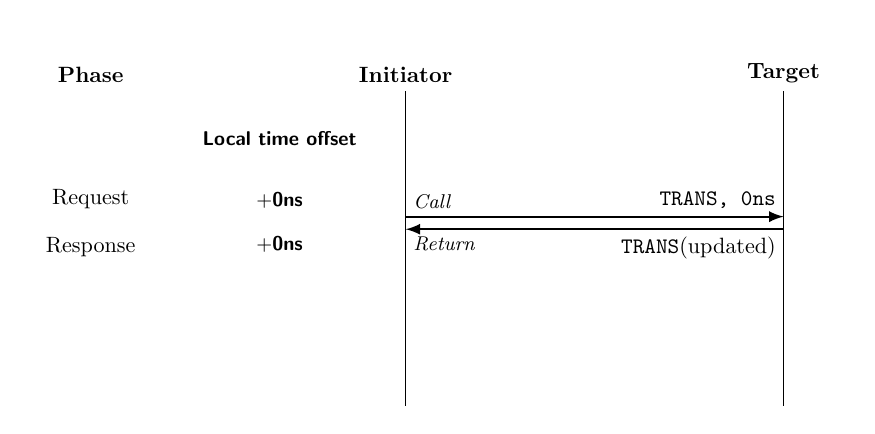
\begin{tikzpicture}[transform shape,scale=0.8]
		\clip (1,0) rectangle (14,6);
%		\draw[help lines] (0,0) grid (15,10);
		\path (2,5) coordinate (phase);
		\path (2,3) coordinate (req);
		\path (2,2.8) coordinate (rsp);
		\path (5,4) coordinate (time);
		\path (5,3) coordinate (0ns);
		\path (5,2.8) coordinate (0nstext);
		\path (7,0) coordinate (llb);
		\path (7,5) coordinate (llt);
		\path (13,0) coordinate (rlb);
		\path (13,5) coordinate (rlt);
		\path (7,3) coordinate (call_left);
		\path (13,3) coordinate (call_right);
		\path (7,2.8) coordinate (ret_left);
		\path (13,2.8) coordinate (ret_right);

		\onslide*<1-> {
		\draw (phase) node[above] {\textbf{Phase}};
		\draw (llb) -- (llt)
			node[above] {\textbf{Initiator}};
		\draw (rlb) -- (rlt)
			node[above] {\textbf{Target}};
		\draw (time) node[above] {\small \textbf{\textsf{Local time offset}}};
		}
		\onslide*<2-> {
		\draw (req) node[above] {Request};
		\draw (0ns) node[above] {\small \textbf{\textsf{$+$0ns}}};
		\draw[thick,-latex] (call_left) -- (call_right);
		\draw (call_left) node[above right] {\small \emph{Call}};
		\draw (call_right) node[above left] {\texttt{\textbf{TRANS, 0ns}}};
		}
		\onslide*<3-> {
		\draw (rsp) node[below] {Response};
		\draw[thick,latex-] (ret_left) -- (ret_right);
		\draw (ret_left) node[below right] {\small \emph{Return}};
		\draw (ret_right) node[below left] {\texttt{\textbf{TRANS}}(updated)};
		\draw (0nstext) node[below] {\small \textbf{\textsf{$+$0ns}}};
		}
	\end{tikzpicture}
\end{figure}
\end{frame}
}

\mode<article>{
Figure~\ref{fig:chart_untimed} shows the message exchange that occur when using the untimed coding style.

\begin{figure}[h]
	\begin{center}
	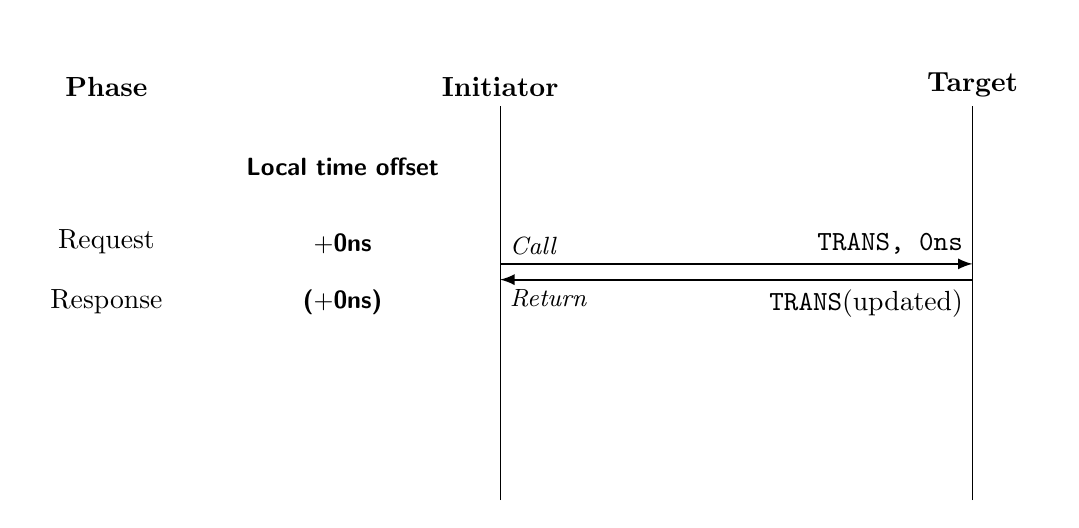
\begin{tikzpicture}
		\clip (1,0) rectangle (14,6);
%		\draw[help lines] (0,0) grid (15,10);
		\path (2,5) coordinate (phase);
		\path (2,3) coordinate (req);
		\path (2,2.8) coordinate (rsp);
		\path (5,4) coordinate (time);
		\path (5,3) coordinate (0ns);
		\path (5,2.8) coordinate (0nstext);
		\path (7,0) coordinate (llb);
		\path (7,5) coordinate (llt);
		\path (13,0) coordinate (rlb);
		\path (13,5) coordinate (rlt);
		\path (7,3) coordinate (call_left);
		\path (13,3) coordinate (call_right);
		\path (7,2.8) coordinate (ret_left);
		\path (13,2.8) coordinate (ret_right);

		\draw (phase) node[above] {\textbf{Phase}};
		\draw (llb) -- (llt)
			node[above] {\textbf{Initiator}};
		\draw (rlb) -- (rlt)
			node[above] {\textbf{Target}};
		\draw (req) node[above] {Request};
		\draw (rsp) node[below] {Response};
		\draw (time) node[above] {\small \textbf{\textsf{Local time offset}}};
		\draw (0ns) node[above] {\small \textbf{\textsf{$+$0ns}}};
		\draw (0nstext) node[below] {\small \textbf{\textsf{($+$0ns)}}};
		\draw[thick,-latex] (call_left) -- (call_right);
		\draw (call_left) node[above right] {\small \emph{Call}};
		\draw (call_right) node[above left] {\texttt{\textbf{TRANS, 0ns}}};
		\draw[thick,latex-] (ret_left) -- (ret_right);
		\draw (ret_left) node[below right] {\small \emph{Return}};
		\draw (ret_right) node[below left] {\texttt{\textbf{TRANS}}(updated)};
	\end{tikzpicture}
	\end{center}
	\caption{Untimed coding style message chart.}
	\label{fig:chart_untimed}
\end{figure}
}

\subsection{Loosely-timed with timing annotation}

\mode<presentation>{

\begin{frame}
	\frametitle{Loosely-timed with timing annotation}

\begin{figure}[h]
	\begin{center}
	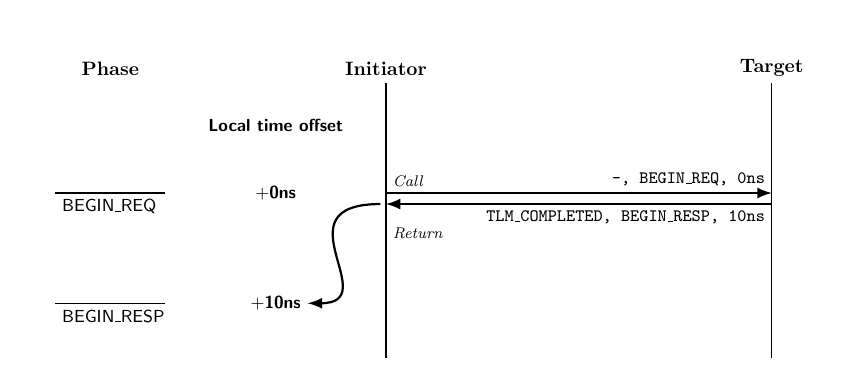
\begin{tikzpicture}[transform shape,scale=0.7]
		\clip (0.5,0) rectangle (15,6);
%		\draw[help lines] (0,0) grid (15,10);
		\path (2,5) coordinate (phase);
		\path (1,3) coordinate (req0);
		\path (3,3) coordinate (req1);
		\path (1,1) coordinate (rsp0);
		\path (3,1) coordinate (rsp1);
		\path (5,4) coordinate (time);
		\path (5,3) coordinate (0ns);
		\path (5,1) coordinate (10ns);
		\path (7,0) coordinate (llb);
		\path (7,5) coordinate (llt);
		\path (14,0) coordinate (rlb);
		\path (14,5) coordinate (rlt);
		\path (7,3) coordinate (call_left);
		\path (14,3) coordinate (call_right);
		\path (7,2.8) coordinate (ret_left);
		\path (14,2.8) coordinate (ret_right);

		\draw (phase) node[above] {\textbf{Phase}};
		\draw (llb) -- (llt)
			node[above] {\textbf{Initiator}};
		\draw (rlb) -- (rlt)
			node[above] {\textbf{Target}};
		\draw (req0) node[below right] {\small \textsf{BEGIN\_REQ}} -- (req1);
		\draw (rsp0) node[below right] {\small \textsf{BEGIN\_RESP}} -- (rsp1);
		\draw (time) node[above] {\small \textbf{\textsf{Local time offset}}};
		\draw (0ns) node {\small \textbf{\textsf{$+$0ns}}};
		\draw (10ns) node(10nstext) {\small \textbf{\textsf{$+$10ns}}};
		\draw[thick,-latex] (call_left) -- (call_right);
		\draw (call_left) node[above right] {\footnotesize \emph{Call}};
		\draw (call_right) node[above left] {\small \texttt{\textbf{-, BEGIN\_REQ, 0ns}}};
		\draw[thick,latex-] (ret_left) -- (ret_right);
		\draw (ret_left) +(0,-0.3) node[below right] {\footnotesize \emph{Return}};
		\draw (ret_right) node[below left] {\small \texttt{\textbf{TLM\_COMPLETED, BEGIN\_RESP, 10ns}}};
		\path (ret_left) +(-2,0) coordinate (control_ret_left);
		\path (10nstext)[above] +(2,0) coordinate (control_10nstext);
		\draw[thick,-latex] (ret_left) +(-0.1,0) .. controls (control_ret_left) and (control_10nstext) .. (10nstext)[above];
	\end{tikzpicture}
	\end{center}
\end{figure}

\end{frame}

}

\mode<article>{
Figure~\ref{fig:chart_lt_with_timing_annotation} shows the message exchange that occur when using the loosely-timed coding style with timing annotation.

\begin{figure}[h]
	\begin{center}
	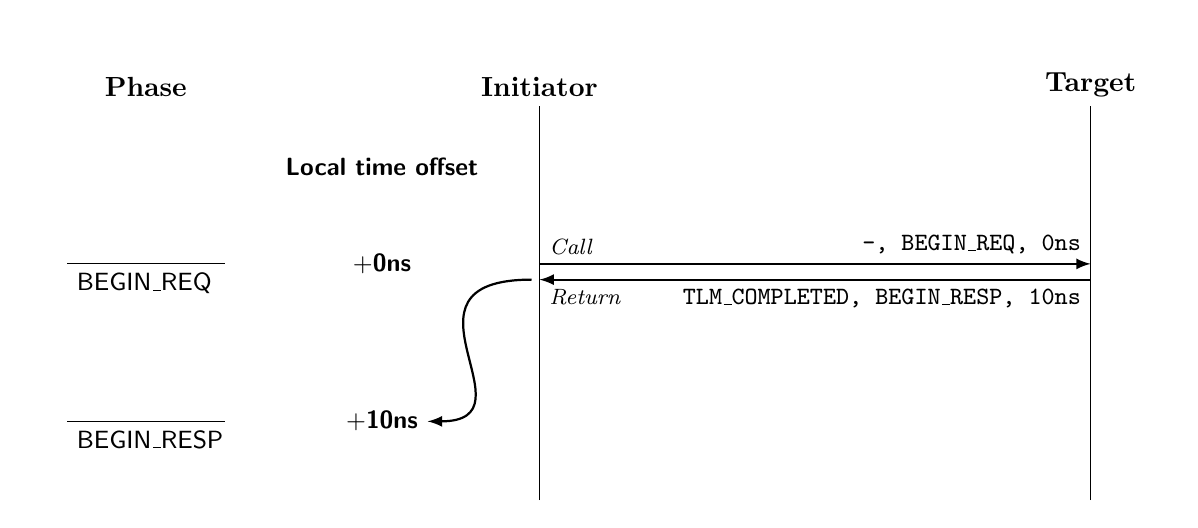
\begin{tikzpicture}
		\clip (0.5,0) rectangle (15,6);
%		\draw[help lines] (0,0) grid (15,10);
		\path (2,5) coordinate (phase);
		\path (1,3) coordinate (req0);
		\path (3,3) coordinate (req1);
		\path (1,1) coordinate (rsp0);
		\path (3,1) coordinate (rsp1);
		\path (5,4) coordinate (time);
		\path (5,3) coordinate (0ns);
		\path (5,1) coordinate (10ns);
		\path (7,0) coordinate (llb);
		\path (7,5) coordinate (llt);
		\path (14,0) coordinate (rlb);
		\path (14,5) coordinate (rlt);
		\path (7,3) coordinate (call_left);
		\path (14,3) coordinate (call_right);
		\path (7,2.8) coordinate (ret_left);
		\path (14,2.8) coordinate (ret_right);

		\draw (phase) node[above] {\textbf{Phase}};
		\draw (llb) -- (llt)
			node[above] {\textbf{Initiator}};
		\draw (rlb) -- (rlt)
			node[above] {\textbf{Target}};
		\draw (req0) node[below right] {\small \textsf{BEGIN\_REQ}} -- (req1);
		\draw (rsp0) node[below right] {\small \textsf{BEGIN\_RESP}} -- (rsp1);
		\draw (time) node[above] {\small \textbf{\textsf{Local time offset}}};
		\draw (0ns) node {\small \textbf{\textsf{$+$0ns}}};
		\draw (10ns) node(10nstext) {\small \textbf{\textsf{$+$10ns}}};
		\draw[thick,-latex] (call_left) -- (call_right);
		\draw (call_left) node[above right] {\footnotesize \emph{Call}};
		\draw (call_right) node[above left] {\small \texttt{\textbf{-, BEGIN\_REQ, 0ns}}};
		\draw[thick,latex-] (ret_left) -- (ret_right);
		\draw (ret_left) node[below right] {\footnotesize \emph{Return}};
		\draw (ret_right) node[below left] {\small \texttt{\textbf{TLM\_COMPLETED, BEGIN\_RESP, 10ns}}};
		\path (ret_left) +(-2,0) coordinate (control_ret_left);
		\path (10nstext)[above] +(2,0) coordinate (control_10nstext);
		\draw[thick,-latex] (ret_left) +(-0.1,0) .. controls (control_ret_left) and (control_10nstext) .. (10nstext)[above];
	\end{tikzpicture}
	\end{center}
	\caption{Loosely-timed coding style with timing annotation message chart.}
	\label{fig:chart_lt_with_timing_annotation}
\end{figure}
}

\clearpage
\subsection{Loosely-timed with sync}

\mode<presentation>{

\begin{frame}
	\frametitle{Loosely-timed with sync}

\begin{figure}[h]
	\begin{center}
	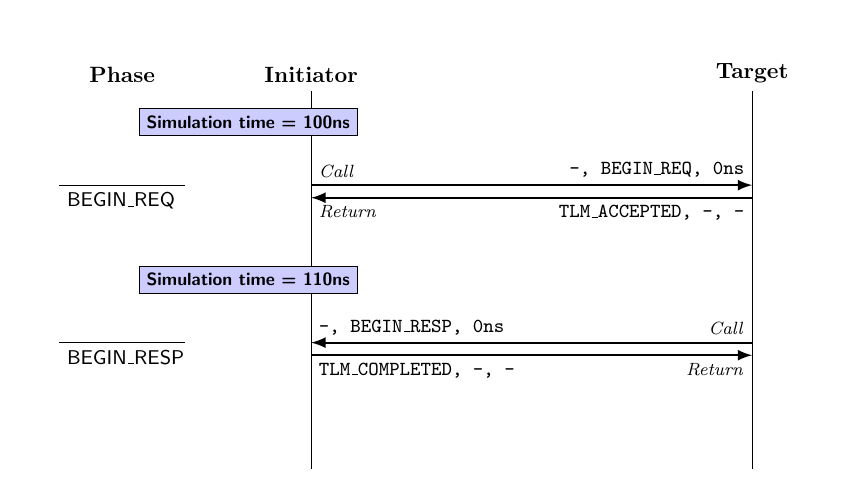
\begin{tikzpicture}[transform shape,scale=0.8]
		\clip (2.5,0) rectangle (15,7);
%		\draw[help lines] (0,0) grid (15,10);
		\path (4,6) coordinate (phase);
		\path (3,4.5) coordinate (req0);
		\path (5,4.5) coordinate (req1);
		\path (3,2) coordinate (rsp0);
		\path (5,2) coordinate (rsp1);
		\path (7,0) coordinate (llb);
		\path (7,6) coordinate (llt);
		\path (14,0) coordinate (rlb);
		\path (14,6) coordinate (rlt);
		\path (7,4.5) coordinate (call_left);
		\path (14,4.5) coordinate (call_right);
		\path (7,4.3) coordinate (ret_left);
		\path (14,4.3) coordinate (ret_right);
		\path (7,2) coordinate (call2_left);
		\path (14,2) coordinate (call2_right);
		\path (7,1.8) coordinate (ret2_left);
		\path (14,1.8) coordinate (ret2_right);

		\draw (phase) node[above] {\textbf{Phase}};
		\draw (llb) -- (llt)
			node[above] {\textbf{Initiator}};
		\draw (rlb) -- (rlt)
			node[above] {\textbf{Target}};
		\draw (req0) node[below right] {\small \textsf{BEGIN\_REQ}} -- (req1);
		\draw (rsp0) node[below right] {\small \textsf{BEGIN\_RESP}} -- (rsp1);
		\draw[thick,-latex] (call_left) -- (call_right);
		\draw (call_left) node[above right] {\footnotesize \emph{Call}};
		\draw (call_right) node[above left] {\small \texttt{\textbf{-, BEGIN\_REQ, 0ns}}};
		\draw[thick,latex-] (ret_left) -- (ret_right);
		\draw (ret_left) node[below right] {\footnotesize \emph{Return}};
		\draw (ret_right) node[below left] {\small \texttt{\textbf{TLM\_ACCEPTED, -, -}}};
		\draw[thick,latex-] (call2_left) -- (call2_right);
		\draw (call2_right) node[above left] {\footnotesize \emph{Call}};
		\draw (call2_left) node[above right] {\small \texttt{\textbf{-, BEGIN\_RESP, 0ns}}};
		\draw[thick,-latex] (ret2_left) -- (ret2_right);
		\draw (ret2_right) node[below left] {\footnotesize \emph{Return}};
		\draw (ret2_left) node[below right] {\small \texttt{\textbf{TLM\_COMPLETED, -, -}}};
		\path (6,5.5) node(100ns) [rectangle,draw,fill=blue!20] {\footnotesize \textsf{\textbf{Simulation time = 100ns}}};
		\path (6,3) node(110ns) [rectangle,draw,fill=blue!20] {\footnotesize \textsf{\textbf{Simulation time = 110ns}}};
	\end{tikzpicture}
	\end{center}
\end{figure}
\end{frame}
}

\mode<article>{
Figure~\ref{fig:chart_lt_with_sync} shows the message exchange that occur when using the loosely-timed coding style with sync.

\begin{figure}[h]
	\begin{center}
	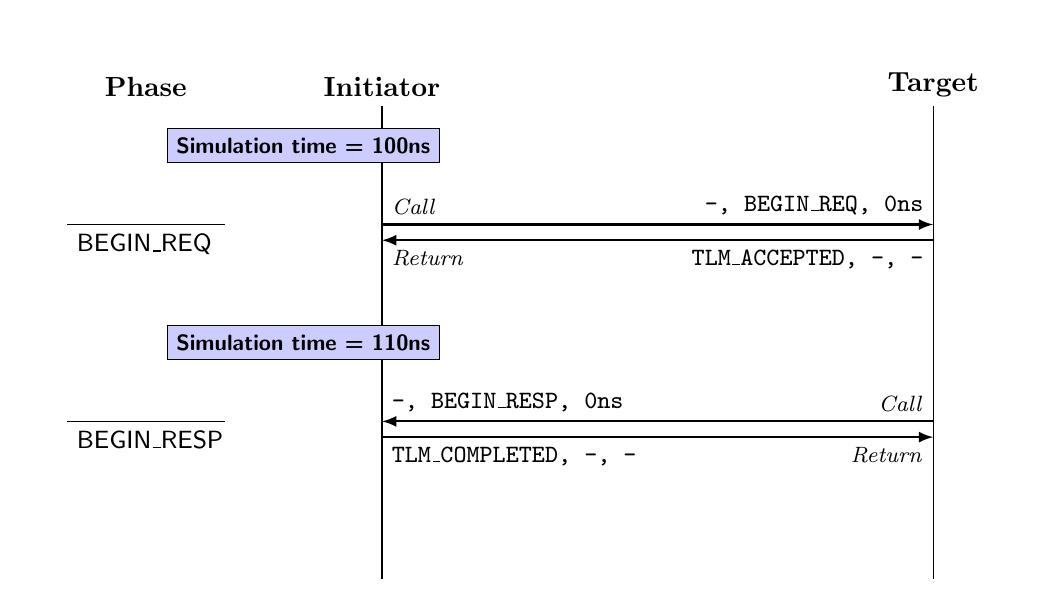
\begin{tikzpicture}
		\clip (2.5,0) rectangle (15,7);
%		\draw[help lines] (0,0) grid (15,10);
		\path (4,6) coordinate (phase);
		\path (3,4.5) coordinate (req0);
		\path (5,4.5) coordinate (req1);
		\path (3,2) coordinate (rsp0);
		\path (5,2) coordinate (rsp1);
		\path (7,0) coordinate (llb);
		\path (7,6) coordinate (llt);
		\path (14,0) coordinate (rlb);
		\path (14,6) coordinate (rlt);
		\path (7,4.5) coordinate (call_left);
		\path (14,4.5) coordinate (call_right);
		\path (7,4.3) coordinate (ret_left);
		\path (14,4.3) coordinate (ret_right);
		\path (7,2) coordinate (call2_left);
		\path (14,2) coordinate (call2_right);
		\path (7,1.8) coordinate (ret2_left);
		\path (14,1.8) coordinate (ret2_right);

		\draw (phase) node[above] {\textbf{Phase}};
		\draw (llb) -- (llt)
			node[above] {\textbf{Initiator}};
		\draw (rlb) -- (rlt)
			node[above] {\textbf{Target}};
		\draw (req0) node[below right] {\small \textsf{BEGIN\_REQ}} -- (req1);
		\draw (rsp0) node[below right] {\small \textsf{BEGIN\_RESP}} -- (rsp1);
		\draw[thick,-latex] (call_left) -- (call_right);
		\draw (call_left) node[above right] {\footnotesize \emph{Call}};
		\draw (call_right) node[above left] {\small \texttt{\textbf{-, BEGIN\_REQ, 0ns}}};
		\draw[thick,latex-] (ret_left) -- (ret_right);
		\draw (ret_left) node[below right] {\footnotesize \emph{Return}};
		\draw (ret_right) node[below left] {\small \texttt{\textbf{TLM\_ACCEPTED, -, -}}};
		\draw[thick,latex-] (call2_left) -- (call2_right);
		\draw (call2_right) node[above left] {\footnotesize \emph{Call}};
		\draw (call2_left) node[above right] {\small \texttt{\textbf{-, BEGIN\_RESP, 0ns}}};
		\draw[thick,-latex] (ret2_left) -- (ret2_right);
		\draw (ret2_right) node[below left] {\footnotesize \emph{Return}};
		\draw (ret2_left) node[below right] {\small \texttt{\textbf{TLM\_COMPLETED, -, -}}};
		\path (6,5.5) node(100ns) [rectangle,draw,fill=blue!20] {\footnotesize \textsf{\textbf{Simulation time = 100ns}}};
		\path (6,3) node(110ns) [rectangle,draw,fill=blue!20] {\footnotesize \textsf{\textbf{Simulation time = 110ns}}};
	\end{tikzpicture}
	\end{center}
	\caption{Loosely-timed coding style with sync message chart.}
	\label{fig:chart_lt_with_sync}
\end{figure}
}

\clearpage
\subsection{Loosely-timed with temporal decoupling}

\mode<presentation>{

\begin{frame}
	\frametitle{Loosely-timed with temporal decoupling}

\begin{figure}[h]
	\begin{center}
	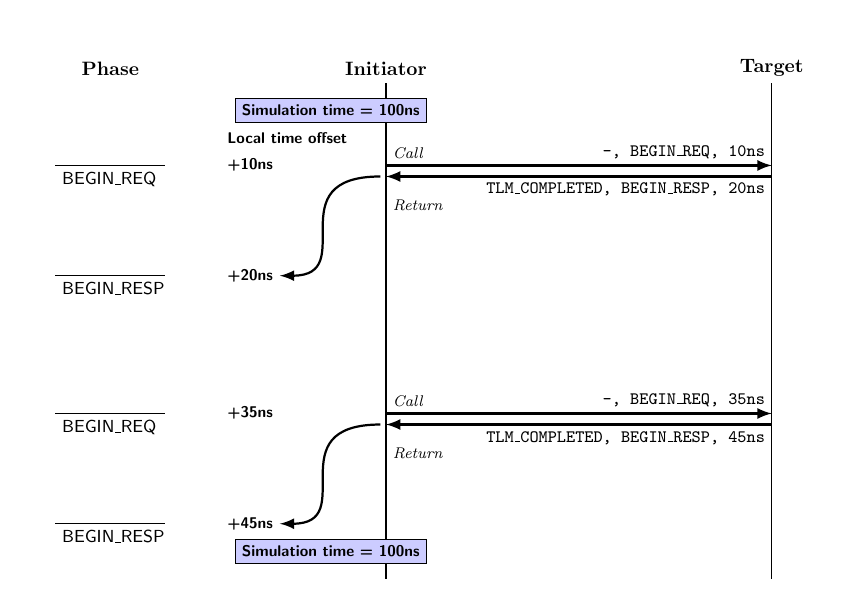
\begin{tikzpicture}[transform shape,scale=0.7]
		\clip (0.5,0) rectangle (15,10);
%		\draw[help lines] (0,0) grid (15,10);
		\path (2,9) coordinate (phase);
		\path (1,7.5) coordinate (req0);
		\path (3,7.5) coordinate (req1);
		\path (1,5.5) coordinate (rsp0);
		\path (3,5.5) coordinate (rsp1);
		\path (1,3) coordinate (req1_0);
		\path (3,3) coordinate (req1_1);
		\path (1,1) coordinate (rsp1_0);
		\path (3,1) coordinate (rsp1_1);
		\path (4,8) node(local_time) [right] {\footnotesize \textsf{\textbf{Local time offset}}};
		\path (4,7.5) node(10ns) [right] {\footnotesize \textsf{\textbf{+10ns}}};
		\path (4,5.5) node(20ns) [right] {\footnotesize \textsf{\textbf{+20ns}}};
		\path (4,3) node(35ns) [right] {\footnotesize \textsf{\textbf{+35ns}}};
		\path (4,1) node(45ns) [right] {\footnotesize \textsf{\textbf{+45ns}}};
		\path (7,0) coordinate (llb);
		\path (7,9) coordinate (llt);
		\path (14,0) coordinate (rlb);
		\path (14,9) coordinate (rlt);
		\path (7,7.5) coordinate (call_left);
		\path (14,7.5) coordinate (call_right);
		\path (7,7.3) coordinate (ret_left);
		\path (14,7.3) coordinate (ret_right);
		\path (7,3) coordinate (call2_left);
		\path (14,3) coordinate (call2_right);
		\path (7,2.8) coordinate (ret2_left);
		\path (14,2.8) coordinate (ret2_right);

		\draw (phase) node[above] {\textbf{Phase}};
		\draw (llb) -- (llt)
			node[above] {\textbf{Initiator}};
		\draw (rlb) -- (rlt)
			node[above] {\textbf{Target}};
		\draw (req0) node[below right] {\small \textsf{BEGIN\_REQ}} -- (req1);
		\draw (rsp0) node[below right] {\small \textsf{BEGIN\_RESP}} -- (rsp1);
		\draw (req1_0) node[below right] {\small \textsf{BEGIN\_REQ}} -- (req1_1);
		\draw (rsp1_0) node[below right] {\small \textsf{BEGIN\_RESP}} -- (rsp1_1);
		\draw[thick,-latex] (call_left) -- (call_right);
		\draw (call_left) node[above right] {\footnotesize \emph{Call}};
		\draw (call_right) node[above left] {\small \texttt{\textbf{-, BEGIN\_REQ, 10ns}}};
		\draw[thick,latex-] (ret_left) -- (ret_right);
		\draw (ret_left) +(0,-0.3) node[below right] {\footnotesize \emph{Return}};
		\draw (ret_right) node[below left] {\small \texttt{\textbf{TLM\_COMPLETED, BEGIN\_RESP, 20ns}}};
		\draw[thick,-latex] (call2_left) -- (call2_right);
		\draw (call2_left) node[above right] {\footnotesize \emph{Call}};
		\draw (call2_right) node[above left] {\small \texttt{\textbf{-, BEGIN\_REQ, 35ns}}};
		\draw[thick,latex-] (ret2_left) -- (ret2_right);
		\draw (ret2_left) +(0,-0.3) node[below right] {\footnotesize \emph{Return}};
		\draw (ret2_right) node[below left] {\small \texttt{\textbf{TLM\_COMPLETED, BEGIN\_RESP, 45ns}}};
		\path (6,8.5) node(100ns) [rectangle,draw,fill=blue!20] {\footnotesize \textsf{\textbf{Simulation time = 100ns}}};
		\path (6,0.5) node(100_ns) [rectangle,draw,fill=blue!20] {\footnotesize \textsf{\textbf{Simulation time = 100ns}}};
		\path (ret_left) +(-2,0) coordinate (control_ret_left);
		\path (20ns) +(2,0) coordinate (control_20ns);
		\draw[thick,-latex] (ret_left) +(-0.1,0) .. controls (control_ret_left) and (control_20ns) .. (20ns)[above];
		\path (ret2_left) +(-2,0) coordinate (control_ret2_left);
		\path (45ns) +(2,0) coordinate (control_45ns);
		\draw[thick,-latex] (ret2_left) +(-0.1,0) .. controls (control_ret2_left) and (control_45ns) .. (45ns)[above];
	\end{tikzpicture}
	\end{center}
\end{figure}
\end{frame}

}

\mode<article>{
Figure~\ref{fig:chart_lt_with_temporal_decoupling} shows the message exchange that occur when using the loosely-timed coding style with temporal decoupling.

\begin{figure}[h]
	\begin{center}
	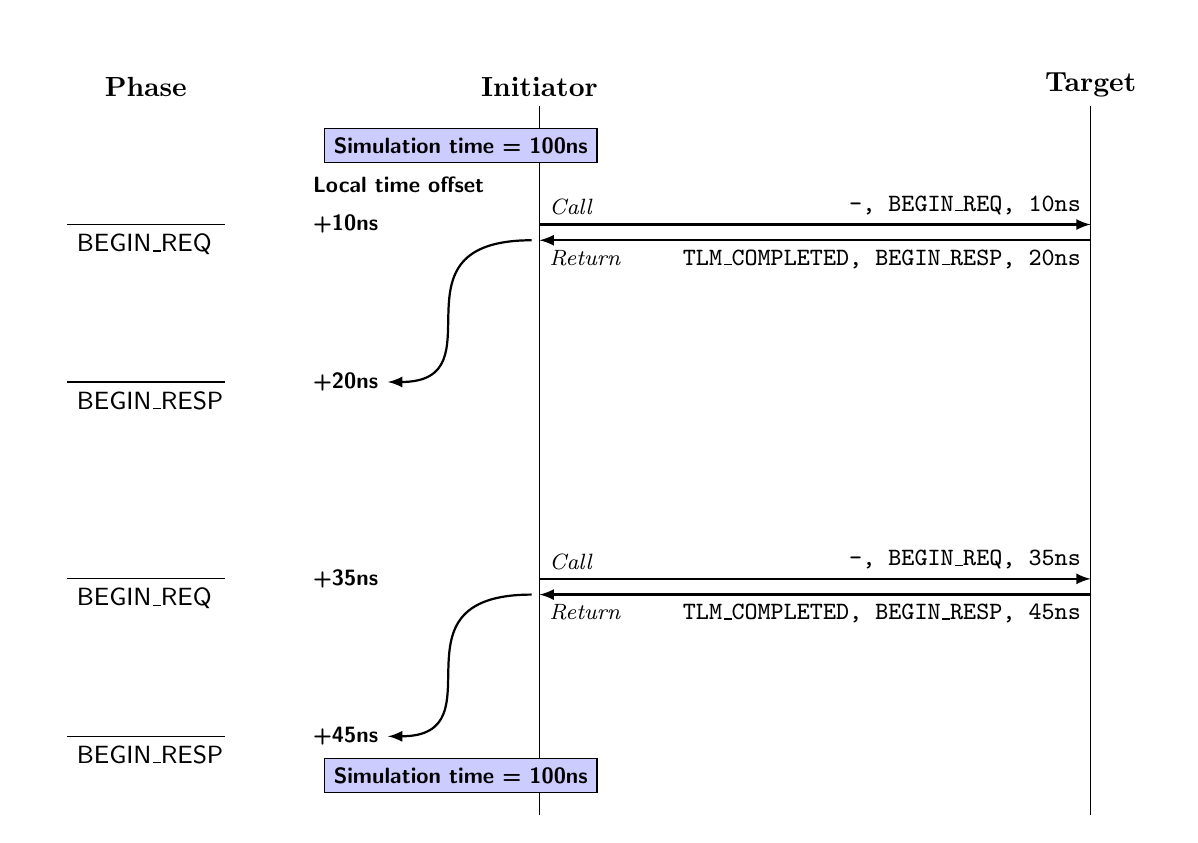
\begin{tikzpicture}
		\clip (0.5,0) rectangle (15,10);
%		\draw[help lines] (0,0) grid (15,10);
		\path (2,9) coordinate (phase);
		\path (1,7.5) coordinate (req0);
		\path (3,7.5) coordinate (req1);
		\path (1,5.5) coordinate (rsp0);
		\path (3,5.5) coordinate (rsp1);
		\path (1,3) coordinate (req1_0);
		\path (3,3) coordinate (req1_1);
		\path (1,1) coordinate (rsp1_0);
		\path (3,1) coordinate (rsp1_1);
		\path (4,8) node(local_time) [right] {\footnotesize \textsf{\textbf{Local time offset}}};
		\path (4,7.5) node(10ns) [right] {\footnotesize \textsf{\textbf{+10ns}}};
		\path (4,5.5) node(20ns) [right] {\footnotesize \textsf{\textbf{+20ns}}};
		\path (4,3) node(35ns) [right] {\footnotesize \textsf{\textbf{+35ns}}};
		\path (4,1) node(45ns) [right] {\footnotesize \textsf{\textbf{+45ns}}};
		\path (7,0) coordinate (llb);
		\path (7,9) coordinate (llt);
		\path (14,0) coordinate (rlb);
		\path (14,9) coordinate (rlt);
		\path (7,7.5) coordinate (call_left);
		\path (14,7.5) coordinate (call_right);
		\path (7,7.3) coordinate (ret_left);
		\path (14,7.3) coordinate (ret_right);
		\path (7,3) coordinate (call2_left);
		\path (14,3) coordinate (call2_right);
		\path (7,2.8) coordinate (ret2_left);
		\path (14,2.8) coordinate (ret2_right);

		\draw (phase) node[above] {\textbf{Phase}};
		\draw (llb) -- (llt)
			node[above] {\textbf{Initiator}};
		\draw (rlb) -- (rlt)
			node[above] {\textbf{Target}};
		\draw (req0) node[below right] {\small \textsf{BEGIN\_REQ}} -- (req1);
		\draw (rsp0) node[below right] {\small \textsf{BEGIN\_RESP}} -- (rsp1);
		\draw (req1_0) node[below right] {\small \textsf{BEGIN\_REQ}} -- (req1_1);
		\draw (rsp1_0) node[below right] {\small \textsf{BEGIN\_RESP}} -- (rsp1_1);
		\draw[thick,-latex] (call_left) -- (call_right);
		\draw (call_left) node[above right] {\footnotesize \emph{Call}};
		\draw (call_right) node[above left] {\small \texttt{\textbf{-, BEGIN\_REQ, 10ns}}};
		\draw[thick,latex-] (ret_left) -- (ret_right);
		\draw (ret_left) node[below right] {\footnotesize \emph{Return}};
		\draw (ret_right) node[below left] {\small \texttt{\textbf{TLM\_COMPLETED, BEGIN\_RESP, 20ns}}};
		\draw[thick,-latex] (call2_left) -- (call2_right);
		\draw (call2_left) node[above right] {\footnotesize \emph{Call}};
		\draw (call2_right) node[above left] {\small \texttt{\textbf{-, BEGIN\_REQ, 35ns}}};
		\draw[thick,latex-] (ret2_left) -- (ret2_right);
		\draw (ret2_left) node[below right] {\footnotesize \emph{Return}};
		\draw (ret2_right) node[below left] {\small \texttt{\textbf{TLM\_COMPLETED, BEGIN\_RESP, 45ns}}};
		\path (6,8.5) node(100ns) [rectangle,draw,fill=blue!20] {\footnotesize \textsf{\textbf{Simulation time = 100ns}}};
		\path (6,0.5) node(100_ns) [rectangle,draw,fill=blue!20] {\footnotesize \textsf{\textbf{Simulation time = 100ns}}};
		\path (ret_left) +(-2,0) coordinate (control_ret_left);
		\path (20ns) +(2,0) coordinate (control_20ns);
		\draw[thick,-latex] (ret_left) +(-0.1,0) .. controls (control_ret_left) and (control_20ns) .. (20ns)[above];
		\path (ret2_left) +(-2,0) coordinate (control_ret2_left);
		\path (45ns) +(2,0) coordinate (control_45ns);
		\draw[thick,-latex] (ret2_left) +(-0.1,0) .. controls (control_ret2_left) and (control_45ns) .. (45ns)[above];
	\end{tikzpicture}
	\end{center}
	\caption{Loosely-timed coding style with temporal decoupling message chart.}
	\label{fig:chart_lt_with_temporal_decoupling}
\end{figure}
}

\clearpage
\subsection{Loosely-timed with temporal decoupling and synchronization-on-demand}

\mode<presentation>{

\begin{frame}
	\frametitle{\scriptsize Loosely-timed with temporal decoupling and synchronization-on-demand}

\begin{figure}[h]
	\begin{center}
	\begin{tikzpicture}[transform shape,scale=0.7]
		\clip (0.5,0) rectangle (15,10);
%		\draw[help lines] (0,0) grid (15,10);
		\path (2,9) coordinate (phase);
		\path (1,7.5) coordinate (req0);
		\path (3,7.5) coordinate (req1);
		\path (1,4) coordinate (rsp0);
		\path (3,4) coordinate (rsp1);
		\path (1,2) coordinate (req1_0);
		\path (3,2) coordinate (req1_1);
		\path (1,1) coordinate (rsp1_0);
		\path (3,1) coordinate (rsp1_1);
		\path (4,8) node(local_time) [right] {\footnotesize \textsf{\textbf{Local time offset}}};
		\path (4,7.5) node(10ns) [right] {\footnotesize \textsf{\textbf{+10ns}}};
		\path (4,6.5) node(wait) [right] {\footnotesize \textsf{\textbf{wait(\ldots)}}};
		\path (4,4) node(0s) [right] {\footnotesize \textsf{\textbf{+0ns}}};
		\path (4,2) node(20ns) [right] {\footnotesize \textsf{\textbf{+20ns}}};
		\path (4,1) node(30ns) [right] {\footnotesize \textsf{\textbf{+30ns}}};
		\path (7,0) coordinate (llb);
		\path (7,9) coordinate (llt);
		\path (14,0) coordinate (rlb);
		\path (14,9) coordinate (rlt);
		\path (7,7.5) coordinate (call_left);
		\path (14,7.5) coordinate (call_right);
		\path (7,7.3) coordinate (ret_left);
		\path (14,7.3) coordinate (ret_right);
		\path (7,4) coordinate (call2_left);
		\path (14,4) coordinate (call2_right);
		\path (7,3.8) coordinate (ret2_left);
		\path (14,3.8) coordinate (ret2_right);
		\path (7,2) coordinate (call3_left);
		\path (14,2) coordinate (call3_right);
		\path (7,1.8) coordinate (ret3_left);
		\path (14,1.8) coordinate (ret3_right);

		\draw (phase) node[above] {\textbf{Phase}};
		\draw (llb) -- (llt)
			node[above] {\textbf{Initiator}};
		\draw (rlb) -- (rlt)
			node[above] {\textbf{Target}};
		\draw (req0) node[below right] {\small \textsf{BEGIN\_REQ}} -- (req1);
		\draw (rsp0) node[below right] {\small \textsf{BEGIN\_RESP}} -- (rsp1);
		\draw (req1_0) node[below right] {\small \textsf{BEGIN\_REQ}} -- (req1_1);
		\draw (rsp1_0) node[below right] {\small \textsf{BEGIN\_RESP}} -- (rsp1_1);
		\draw[thick,-latex] (call_left) -- (call_right);
		\draw (call_left) node[above right] {\footnotesize \emph{Call}};
		\draw (call_right) node[above left] {\small \texttt{\textbf{-, BEGIN\_REQ, 10ns}}};
		\draw[thick,latex-] (ret_left) -- (ret_right);
		\draw (ret_left) node[below right] {\footnotesize \emph{Return}};
		\draw (ret_right) node[below left] {\small \texttt{\textbf{TLM\_ACCEPTED, -, -}}};
		\draw[thick,latex-] (call2_left) -- (call2_right);
		\draw (call2_right) node[above left] {\footnotesize \emph{Call}};
		\draw (call2_left) node[above right] {\small \texttt{\textbf{-, BEGIN\_RESP, 0ns}}};
		\draw[thick,-latex] (ret2_left) -- (ret2_right);
		\draw (ret2_right) node[below left] {\footnotesize \emph{Return}};
		\draw (ret2_left) node[below right] {\small \texttt{\textbf{TLM\_COMPLETED, -, -}}};
		\draw[thick,-latex] (call3_left) -- (call3_right);
		\draw (call3_left) node[above right] {\footnotesize \emph{Call}};
		\draw (call3_right) node[above left] {\small \texttt{\textbf{-, BEGIN\_REQ, 20ns}}};
		\draw[thick,latex-] (ret3_left) -- (ret3_right);
		\draw (ret3_left) +(0,-0.3) node[below right] {\footnotesize \emph{Return}};
		\draw (ret3_right) node[below left] {\small \texttt{\textbf{TLM\_COMPLETED, BEGIN\_RESP, 30ns}}};
		\path (6,8.5) node(5us) [rectangle,draw,fill=blue!20] {\footnotesize \textsf{\textbf{Simulation time = 5us}}};
		\path (6,5.5) node(6us1) [rectangle,draw,fill=blue!20] {\footnotesize \textsf{\textbf{Simulation time = 6us}}};
		\path (6,0.25) node(6us2) [rectangle,draw,fill=blue!20] {\footnotesize \textsf{\textbf{Simulation time = 6us}}};
		\path (ret_left) +(-1.5,0) coordinate (control_ret_left);
		\path (wait) +(1.5,0) coordinate (control_wait);
		\draw[thick,-latex] (ret_left) +(-0.1,0) .. controls (control_ret_left) and (control_wait) .. (wait)[above];
		\path (ret3_left) +(-2,0) coordinate (control_ret3_left);
		\path (45ns) +(2,0) coordinate (control_45ns);
		\draw[thick,-latex] (ret3_left) +(-0.1,0) .. controls (control_ret3_left) and (control_45ns) .. (45ns)[above];
	\end{tikzpicture}
	\end{center}
\end{figure}

\end{frame}

}

\mode<article>{
Figure~\ref{fig:chart_lt_with_temporal_decoupling_and_sync_on_demand} shows the message exchange that occur when using the loosely-timed coding style with temporal decoupling and synchronization-on-demand.

\begin{figure}[h]
	\begin{center}
	\begin{tikzpicture}
		\clip (0.5,0) rectangle (15,10);
%		\draw[help lines] (0,0) grid (15,10);
		\path (2,9) coordinate (phase);
		\path (1,7.5) coordinate (req0);
		\path (3,7.5) coordinate (req1);
		\path (1,4) coordinate (rsp0);
		\path (3,4) coordinate (rsp1);
		\path (1,2) coordinate (req1_0);
		\path (3,2) coordinate (req1_1);
		\path (1,1) coordinate (rsp1_0);
		\path (3,1) coordinate (rsp1_1);
		\path (4,8) node(local_time) [right] {\footnotesize \textsf{\textbf{Local time offset}}};
		\path (4,7.5) node(10ns) [right] {\footnotesize \textsf{\textbf{+10ns}}};
		\path (4,6.5) node(wait) [right] {\footnotesize \textsf{\textbf{wait(\ldots)}}};
		\path (4,4) node(0s) [right] {\footnotesize \textsf{\textbf{+0ns}}};
		\path (4,2) node(20ns) [right] {\footnotesize \textsf{\textbf{+20ns}}};
		\path (4,1) node(30ns) [right] {\footnotesize \textsf{\textbf{+30ns}}};
		\path (7,0) coordinate (llb);
		\path (7,9) coordinate (llt);
		\path (14,0) coordinate (rlb);
		\path (14,9) coordinate (rlt);
		\path (7,7.5) coordinate (call_left);
		\path (14,7.5) coordinate (call_right);
		\path (7,7.3) coordinate (ret_left);
		\path (14,7.3) coordinate (ret_right);
		\path (7,4) coordinate (call2_left);
		\path (14,4) coordinate (call2_right);
		\path (7,3.8) coordinate (ret2_left);
		\path (14,3.8) coordinate (ret2_right);
		\path (7,2) coordinate (call3_left);
		\path (14,2) coordinate (call3_right);
		\path (7,1.8) coordinate (ret3_left);
		\path (14,1.8) coordinate (ret3_right);

		\draw (phase) node[above] {\textbf{Phase}};
		\draw (llb) -- (llt)
			node[above] {\textbf{Initiator}};
		\draw (rlb) -- (rlt)
			node[above] {\textbf{Target}};
		\draw (req0) node[below right] {\small \textsf{BEGIN\_REQ}} -- (req1);
		\draw (rsp0) node[below right] {\small \textsf{BEGIN\_RESP}} -- (rsp1);
		\draw (req1_0) node[below right] {\small \textsf{BEGIN\_REQ}} -- (req1_1);
		\draw (rsp1_0) node[below right] {\small \textsf{BEGIN\_RESP}} -- (rsp1_1);
		\draw[thick,-latex] (call_left) -- (call_right);
		\draw (call_left) node[above right] {\footnotesize \emph{Call}};
		\draw (call_right) node[above left] {\small \texttt{\textbf{-, BEGIN\_REQ, 10ns}}};
		\draw[thick,latex-] (ret_left) -- (ret_right);
		\draw (ret_left) node[below right] {\footnotesize \emph{Return}};
		\draw (ret_right) node[below left] {\small \texttt{\textbf{TLM\_ACCEPTED, -, -}}};
		\draw[thick,latex-] (call2_left) -- (call2_right);
		\draw (call2_right) node[above left] {\footnotesize \emph{Call}};
		\draw (call2_left) node[above right] {\small \texttt{\textbf{-, BEGIN\_RESP, 0ns}}};
		\draw[thick,-latex] (ret2_left) -- (ret2_right);
		\draw (ret2_right) node[below left] {\footnotesize \emph{Return}};
		\draw (ret2_left) node[below right] {\small \texttt{\textbf{TLM\_COMPLETED, -, -}}};
		\draw[thick,-latex] (call3_left) -- (call3_right);
		\draw (call3_left) node[above right] {\footnotesize \emph{Call}};
		\draw (call3_right) node[above left] {\small \texttt{\textbf{-, BEGIN\_REQ, 20ns}}};
		\draw[thick,latex-] (ret3_left) -- (ret3_right);
		\draw (ret3_left) node[below right] {\footnotesize \emph{Return}};
		\draw (ret3_right) node[below left] {\small \texttt{\textbf{TLM\_COMPLETED, BEGIN\_RESP, 30ns}}};
		\path (6,8.5) node(5us) [rectangle,draw,fill=blue!20] {\footnotesize \textsf{\textbf{Simulation time = 5us}}};
		\path (6,5.5) node(6us1) [rectangle,draw,fill=blue!20] {\footnotesize \textsf{\textbf{Simulation time = 6us}}};
		\path (6,0.25) node(6us2) [rectangle,draw,fill=blue!20] {\footnotesize \textsf{\textbf{Simulation time = 6us}}};
		\path (ret_left) +(-1.5,0) coordinate (control_ret_left);
		\path (wait) +(1.5,0) coordinate (control_wait);
		\draw[thick,-latex] (ret_left) +(-0.1,0) .. controls (control_ret_left) and (control_wait) .. (wait)[above];
		\path (ret3_left) +(-2,0) coordinate (control_ret3_left);
		\path (45ns) +(2,0) coordinate (control_45ns);
		\draw[thick,-latex] (ret3_left) +(-0.1,0) .. controls (control_ret3_left) and (control_45ns) .. (45ns)[above];
	\end{tikzpicture}
	\end{center}
	\caption{Loosely-timed coding style with temporal decoupling and synchronization-on-demand message chart.}
	\label{fig:chart_lt_with_temporal_decoupling_and_sync_on_demand}
\end{figure}
}

\clearpage
\subsection{Loosely-timed with temporal decoupling and quantum}

\mode<presentation>{

\begin{frame}
	\frametitle{\small Loosely-timed with temporal decoupling and quantum}

\begin{figure}[h]
	\begin{center}
	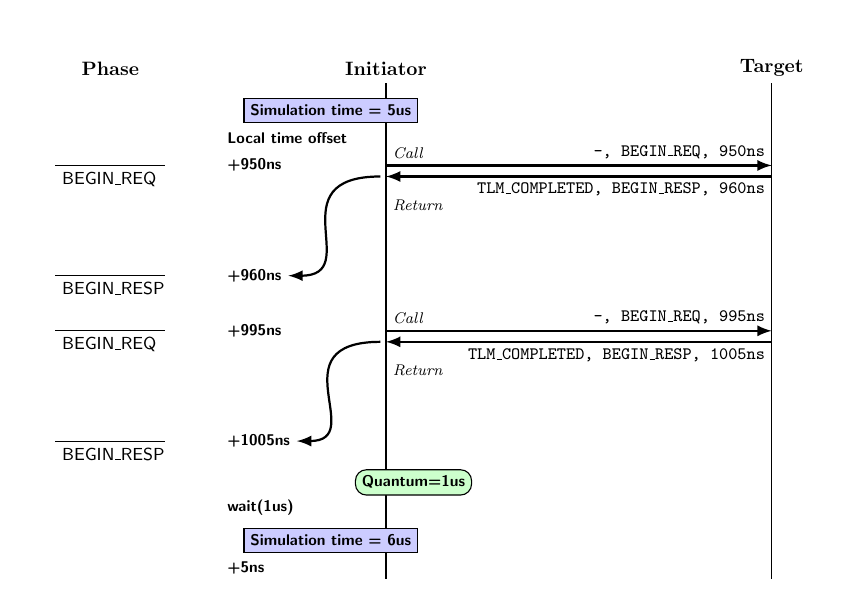
\begin{tikzpicture}[transform shape,scale=0.7]
		\clip (0.5,0) rectangle (15,10);
%		\draw[help lines] (0,0) grid (15,10);
		\path (2,9) coordinate (phase);
		\path (1,7.5) coordinate (req0);
		\path (3,7.5) coordinate (req1);
		\path (1,5.5) coordinate (rsp0);
		\path (3,5.5) coordinate (rsp1);
		\path (1,4.5) coordinate (req1_0);
		\path (3,4.5) coordinate (req1_1);
		\path (1,2.5) coordinate (rsp1_0);
		\path (3,2.5) coordinate (rsp1_1);
		\path (4,8) node(local_time) [right] {\footnotesize \textsf{\textbf{Local time offset}}};
		\path (4,7.5) node(10ns) [right] {\footnotesize \textsf{\textbf{+950ns}}};
		\path (4,5.5) node(20ns) [right] {\footnotesize \textsf{\textbf{+960ns}}};
		\path (4,4.5) node(35ns) [right] {\footnotesize \textsf{\textbf{+995ns}}};
		\path (4,2.5) node(45ns) [right] {\footnotesize \textsf{\textbf{+1005ns}}};
		\path (4,1.3) node(wait) [right] {\footnotesize \textsf{\textbf{wait(1us)}}};
		\path (4,0.2) node(5ns) [right] {\footnotesize \textsf{\textbf{+5ns}}};
		\path (7,0) coordinate (llb);
		\path (7,9) coordinate (llt);
		\path (14,0) coordinate (rlb);
		\path (14,9) coordinate (rlt);
		\path (7,7.5) coordinate (call_left);
		\path (14,7.5) coordinate (call_right);
		\path (7,7.3) coordinate (ret_left);
		\path (14,7.3) coordinate (ret_right);
		\path (7,4.5) coordinate (call2_left);
		\path (14,4.5) coordinate (call2_right);
		\path (7,4.3) coordinate (ret2_left);
		\path (14,4.3) coordinate (ret2_right);

		\draw (phase) node[above] {\textbf{Phase}};
		\draw (llb) -- (llt)
			node[above] {\textbf{Initiator}};
		\draw (rlb) -- (rlt)
			node[above] {\textbf{Target}};
		\draw (req0) node[below right] {\small \textsf{BEGIN\_REQ}} -- (req1);
		\draw (rsp0) node[below right] {\small \textsf{BEGIN\_RESP}} -- (rsp1);
		\draw (req1_0) node[below right] {\small \textsf{BEGIN\_REQ}} -- (req1_1);
		\draw (rsp1_0) node[below right] {\small \textsf{BEGIN\_RESP}} -- (rsp1_1);
		\draw[thick,-latex] (call_left) -- (call_right);
		\draw (call_left) node[above right] {\footnotesize \emph{Call}};
		\draw (call_right) node[above left] {\small \texttt{\textbf{-, BEGIN\_REQ, 950ns}}};
		\draw[thick,latex-] (ret_left) -- (ret_right);
		\draw (ret_left) +(0,-0.3) node[below right] {\footnotesize \emph{Return}};
		\draw (ret_right) node[below left] {\small \texttt{\textbf{TLM\_COMPLETED, BEGIN\_RESP, 960ns}}};
		\draw[thick,-latex] (call2_left) -- (call2_right);
		\draw (call2_left) node[above right] {\footnotesize \emph{Call}};
		\draw (call2_right) node[above left] {\small \texttt{\textbf{-, BEGIN\_REQ, 995ns}}};
		\draw[thick,latex-] (ret2_left) -- (ret2_right);
		\draw (ret2_left) +(0,-0.3) node[below right] {\footnotesize \emph{Return}};
		\draw (ret2_right) node[below left] {\small \texttt{\textbf{TLM\_COMPLETED, BEGIN\_RESP, 1005ns}}};
		\path (6,8.5) node(100ns) [rectangle,draw,fill=blue!20] {\footnotesize \textsf{\textbf{Simulation time = 5us}}};
		\path (6,0.7) node(110ns) [rectangle,draw,fill=blue!20] {\footnotesize \textsf{\textbf{Simulation time = 6us}}};
		\path (7.5,1.75) node(quantum) [rectangle,rounded corners,draw,fill=green!20] {\footnotesize \textsf{\textbf{Quantum=1us}}};
		\path (ret_left) +(-2,0) coordinate (control_ret_left);
		\path (20ns) +(2,0) coordinate (control_20ns);
		\draw[thick,-latex] (ret_left) +(-0.1,0) .. controls (control_ret_left) and (control_20ns) .. (20ns)[above];
		\path (ret2_left) +(-2,0) coordinate (control_ret2_left);
		\path (45ns) +(2,0) coordinate (control_45ns);
		\draw[thick,-latex] (ret2_left) +(-0.1,0) .. controls (control_ret2_left) and (control_45ns) .. (45ns)[above];
	\end{tikzpicture}
	\end{center}
\end{figure}
\end{frame}

}

\mode<article>{
Figure~\ref{fig:chart_lt_with_temporal_decoupling_and_quantum} shows the message exchange that occur when using the loosely-timed coding style and quantum.

\begin{figure}[h]
	\begin{center}
	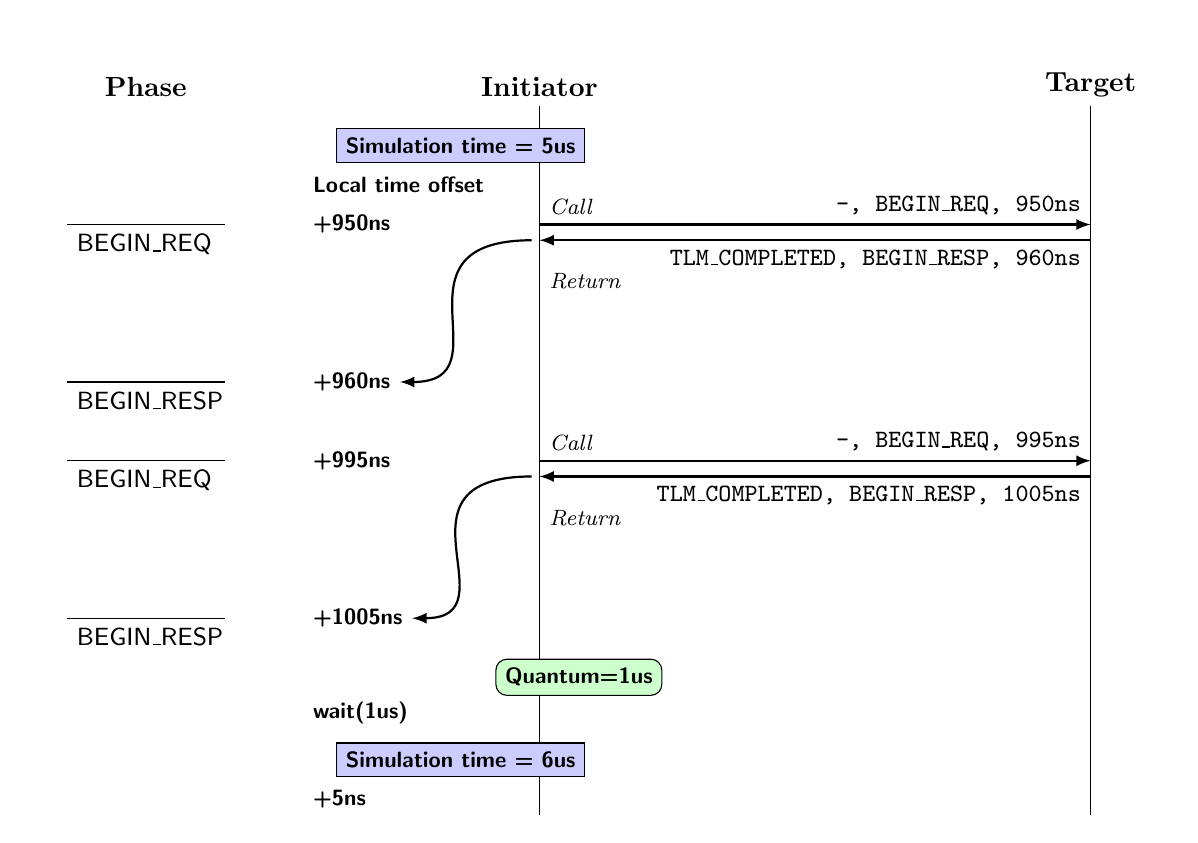
\begin{tikzpicture}
		\clip (0.5,0) rectangle (15,10);
%		\draw[help lines] (0,0) grid (15,10);
		\path (2,9) coordinate (phase);
		\path (1,7.5) coordinate (req0);
		\path (3,7.5) coordinate (req1);
		\path (1,5.5) coordinate (rsp0);
		\path (3,5.5) coordinate (rsp1);
		\path (1,4.5) coordinate (req1_0);
		\path (3,4.5) coordinate (req1_1);
		\path (1,2.5) coordinate (rsp1_0);
		\path (3,2.5) coordinate (rsp1_1);
		\path (4,8) node(local_time) [right] {\footnotesize \textsf{\textbf{Local time offset}}};
		\path (4,7.5) node(10ns) [right] {\footnotesize \textsf{\textbf{+950ns}}};
		\path (4,5.5) node(20ns) [right] {\footnotesize \textsf{\textbf{+960ns}}};
		\path (4,4.5) node(35ns) [right] {\footnotesize \textsf{\textbf{+995ns}}};
		\path (4,2.5) node(45ns) [right] {\footnotesize \textsf{\textbf{+1005ns}}};
		\path (4,1.3) node(wait) [right] {\footnotesize \textsf{\textbf{wait(1us)}}};
		\path (4,0.2) node(5ns) [right] {\footnotesize \textsf{\textbf{+5ns}}};
		\path (7,0) coordinate (llb);
		\path (7,9) coordinate (llt);
		\path (14,0) coordinate (rlb);
		\path (14,9) coordinate (rlt);
		\path (7,7.5) coordinate (call_left);
		\path (14,7.5) coordinate (call_right);
		\path (7,7.3) coordinate (ret_left);
		\path (14,7.3) coordinate (ret_right);
		\path (7,4.5) coordinate (call2_left);
		\path (14,4.5) coordinate (call2_right);
		\path (7,4.3) coordinate (ret2_left);
		\path (14,4.3) coordinate (ret2_right);

		\draw (phase) node[above] {\textbf{Phase}};
		\draw (llb) -- (llt)
			node[above] {\textbf{Initiator}};
		\draw (rlb) -- (rlt)
			node[above] {\textbf{Target}};
		\draw (req0) node[below right] {\small \textsf{BEGIN\_REQ}} -- (req1);
		\draw (rsp0) node[below right] {\small \textsf{BEGIN\_RESP}} -- (rsp1);
		\draw (req1_0) node[below right] {\small \textsf{BEGIN\_REQ}} -- (req1_1);
		\draw (rsp1_0) node[below right] {\small \textsf{BEGIN\_RESP}} -- (rsp1_1);
		\draw[thick,-latex] (call_left) -- (call_right);
		\draw (call_left) node[above right] {\footnotesize \emph{Call}};
		\draw (call_right) node[above left] {\small \texttt{\textbf{-, BEGIN\_REQ, 950ns}}};
		\draw[thick,latex-] (ret_left) -- (ret_right);
		\draw (ret_left) +(0,-0.3) node[below right] {\footnotesize \emph{Return}};
		\draw (ret_right) node[below left] {\small \texttt{\textbf{TLM\_COMPLETED, BEGIN\_RESP, 960ns}}};
		\draw[thick,-latex] (call2_left) -- (call2_right);
		\draw (call2_left) node[above right] {\footnotesize \emph{Call}};
		\draw (call2_right) node[above left] {\small \texttt{\textbf{-, BEGIN\_REQ, 995ns}}};
		\draw[thick,latex-] (ret2_left) -- (ret2_right);
		\draw (ret2_left) +(0,-0.3) node[below right] {\footnotesize \emph{Return}};
		\draw (ret2_right) node[below left] {\small \texttt{\textbf{TLM\_COMPLETED, BEGIN\_RESP, 1005ns}}};
		\path (6,8.5) node(100ns) [rectangle,draw,fill=blue!20] {\footnotesize \textsf{\textbf{Simulation time = 5us}}};
		\path (6,0.7) node(110ns) [rectangle,draw,fill=blue!20] {\footnotesize \textsf{\textbf{Simulation time = 6us}}};
		\path (7.5,1.75) node(quantum) [rectangle,rounded corners,draw,fill=green!20] {\footnotesize \textsf{\textbf{Quantum=1us}}};
		\path (ret_left) +(-2,0) coordinate (control_ret_left);
		\path (20ns) +(2,0) coordinate (control_20ns);
		\draw[thick,-latex] (ret_left) +(-0.1,0) .. controls (control_ret_left) and (control_20ns) .. (20ns)[above];
		\path (ret2_left) +(-2,0) coordinate (control_ret2_left);
		\path (45ns) +(2,0) coordinate (control_45ns);
		\draw[thick,-latex] (ret2_left) +(-0.1,0) .. controls (control_ret2_left) and (control_45ns) .. (45ns)[above];
	\end{tikzpicture}
	\end{center}
	\caption{Loosely-timed coding style with temporal decoupling and quantum message chart.}
	\label{fig:chart_lt_with_temporal_decoupling_and_quantum}
\end{figure}
}

\clearpage
\subsection{Approximately-timed using backward path}

\mode<presentation>{

\begin{frame}
	\frametitle{Approximately-timed using backward path}

\begin{figure}[h]
	\begin{center}
	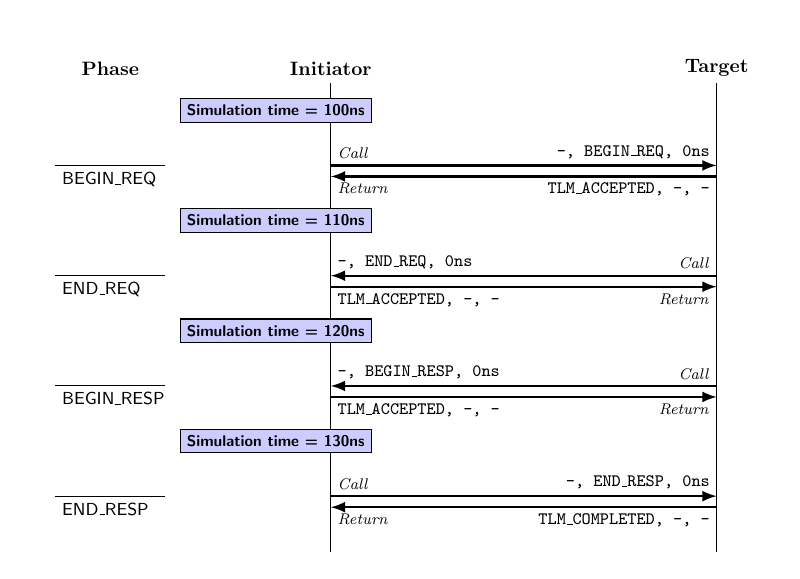
\begin{tikzpicture}[transform shape,scale=0.7]
		\clip (1.5,10.5) rectangle (15,20);
%		\draw[help lines] (0,0) grid (15,20);
		\path (3,19) coordinate (phase);
		\path (7,0) coordinate (llb);
		\path (7,19) coordinate (llt);
		\path (14,0) coordinate (rlb);
		\path (14,19) coordinate (rlt);
		
		\path (6,18.5) coordinate (100ns);
		\path (2,17.5) coordinate (breq_l);
		\path (4,17.5) coordinate (breq_r);
		\path (7,17.5) coordinate (breq_call_l);
		\path (14,17.5) coordinate (breq_call_r);
		\path (7,17.3) coordinate (breq_ret_l);
		\path (14,17.3) coordinate (breq_ret_r);

		\path (6,16.5) coordinate (110ns);
		\path (2,15.5) coordinate (ereq_l);
		\path (4,15.5) coordinate (ereq_r);
		\path (7,15.5) coordinate (ereq_call_l);
		\path (14,15.5) coordinate (ereq_call_r);
		\path (7, 15.3) coordinate (ereq_ret_l);
		\path (14,15.3) coordinate (ereq_ret_r);

		\path (6,14.5) coordinate (120ns);
		\path (2,13.5) coordinate (bresp_l);
		\path (4,13.5) coordinate (bresp_r);
		\path (7,13.5) coordinate (bresp_call_l);
		\path (14,13.5) coordinate (bresp_call_r);
		\path (7,13.3) coordinate (bresp_ret_l);
		\path (14,13.3) coordinate (bresp_ret_r);

		\path (6,12.5) coordinate (130ns);
		\path (2,11.5) coordinate (eresp_l);
		\path (4,11.5) coordinate (eresp_r);
		\path (7,11.5) coordinate (eresp_call_l);
		\path (14,11.5) coordinate (eresp_call_r);
		\path (7,11.3) coordinate (eresp_ret_l);
		\path (14,11.3) coordinate (eresp_ret_r);

		\draw (phase) node[above] {\textbf{Phase}};
		\draw (llb) -- (llt)
			node[above] {\textbf{Initiator}};
		\draw (rlb) -- (rlt)
			node[above] {\textbf{Target}};

		\draw (100ns) node [rectangle,draw,fill=blue!20] {\footnotesize \textsf{\textbf{Simulation time = 100ns}}};
		\draw (breq_l) node[below right] {\small \textsf{BEGIN\_REQ}} -- (breq_r);
		\draw[thick,-latex] (breq_call_l) -- (breq_call_r);
		\draw (breq_call_l) node[above right] {\footnotesize \emph{Call}};
		\draw (breq_call_r) node[above left] {\small \texttt{\textbf{-, BEGIN\_REQ, 0ns}}};
		\draw[thick,latex-] (breq_ret_l) -- (breq_ret_r);
		\draw (breq_ret_l) node[below right] {\footnotesize \emph{Return}};
		\draw (breq_ret_r) node[below left] {\small \texttt{\textbf{TLM\_ACCEPTED, -, -}}};

		\draw (110ns) node [rectangle,draw,fill=blue!20] {\footnotesize \textsf{\textbf{Simulation time = 110ns}}};
		\draw (ereq_l) node[below right] {\small \textsf{END\_REQ}} -- (ereq_r);
		\draw[thick,latex-] (ereq_call_l) -- (ereq_call_r);
		\draw (ereq_call_r) node[above left] {\footnotesize \emph{Call}};
		\draw (ereq_call_l) node[above right] {\small \texttt{\textbf{-, END\_REQ, 0ns}}};
		\draw[thick,-latex] (ereq_ret_l) -- (ereq_ret_r);
		\draw (ereq_ret_r) node[below left] {\footnotesize \emph{Return}};
		\draw (ereq_ret_l) node[below right] {\small \texttt{\textbf{TLM\_ACCEPTED, -, -}}};

		\draw (120ns) node [rectangle,draw,fill=blue!20] {\footnotesize \textsf{\textbf{Simulation time = 120ns}}};
		\draw (bresp_l) node[below right] {\small \textsf{BEGIN\_RESP}} -- (bresp_r);
		\draw[thick,latex-] (bresp_call_l) -- (bresp_call_r);
		\draw (bresp_call_r) node[above left] {\footnotesize \emph{Call}};
		\draw (bresp_call_l) node[above right] {\small \texttt{\textbf{-, BEGIN\_RESP, 0ns}}};
		\draw[thick,-latex] (bresp_ret_l) -- (bresp_ret_r);
		\draw (bresp_ret_r) node[below left] {\footnotesize \emph{Return}};
		\draw (bresp_ret_l) node[below right] {\small \texttt{\textbf{TLM\_ACCEPTED, -, -}}};

		\draw (130ns) node [rectangle,draw,fill=blue!20] {\footnotesize \textsf{\textbf{Simulation time = 130ns}}};
		\draw (eresp_l) node[below right] {\small \textsf{END\_RESP}} -- (eresp_r);
		\draw[thick,-latex] (eresp_call_l) -- (eresp_call_r);
		\draw (eresp_call_l) node[above right] {\footnotesize \emph{Call}};
		\draw (eresp_call_r) node[above left] {\small \texttt{\textbf{-, END\_RESP, 0ns}}};
		\draw[thick,latex-] (eresp_ret_l) -- (eresp_ret_r);
		\draw (eresp_ret_l) node[below right] {\footnotesize \emph{Return}};
		\draw (eresp_ret_r) node[below left] {\small \texttt{\textbf{TLM\_COMPLETED, -, -}}};

	\end{tikzpicture}
	\end{center}
\end{figure}


\end{frame}

}

\mode<article>{
Figure~\ref{fig:chart_at_using_backward_path} shows the message exchange that occur when using the approximately-timed coding style using the backward path.

\begin{figure}[h]
	\begin{center}
	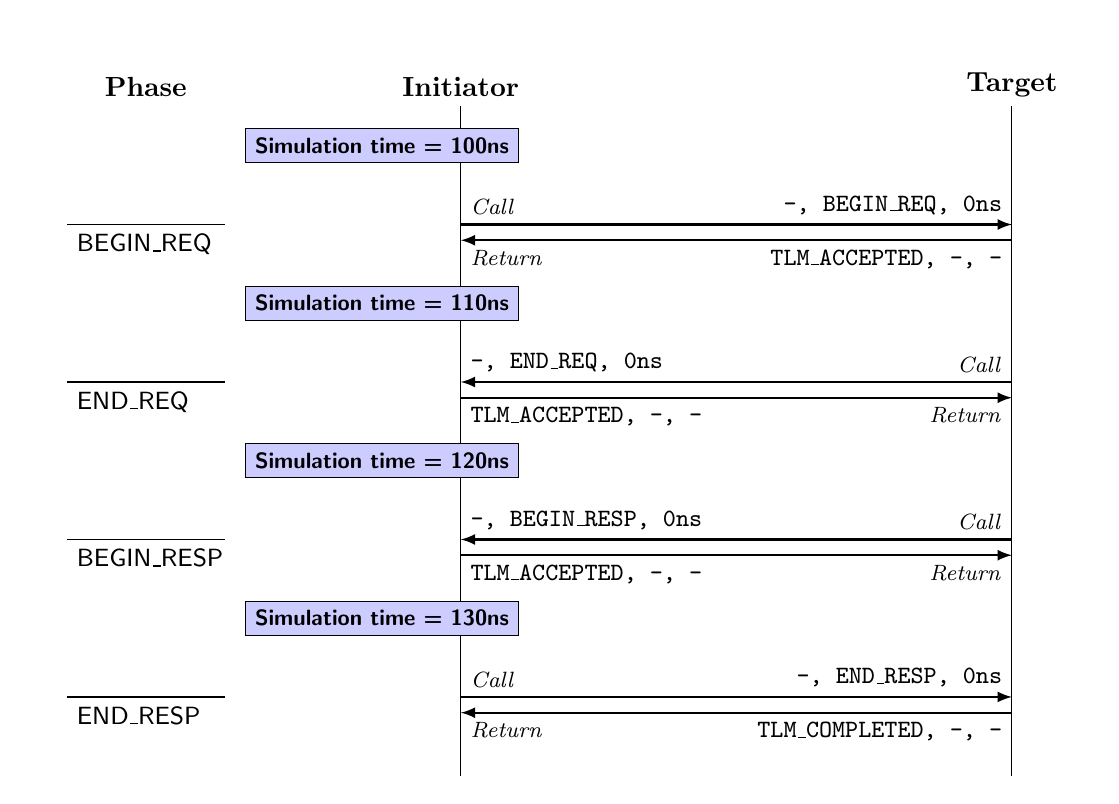
\begin{tikzpicture}
		\clip (1.5,10.5) rectangle (15,20);
%		\draw[help lines] (0,0) grid (15,20);
		\path (3,19) coordinate (phase);
		\path (7,0) coordinate (llb);
		\path (7,19) coordinate (llt);
		\path (14,0) coordinate (rlb);
		\path (14,19) coordinate (rlt);
		
		\path (6,18.5) coordinate (100ns);
		\path (2,17.5) coordinate (breq_l);
		\path (4,17.5) coordinate (breq_r);
		\path (7,17.5) coordinate (breq_call_l);
		\path (14,17.5) coordinate (breq_call_r);
		\path (7,17.3) coordinate (breq_ret_l);
		\path (14,17.3) coordinate (breq_ret_r);

		\path (6,16.5) coordinate (110ns);
		\path (2,15.5) coordinate (ereq_l);
		\path (4,15.5) coordinate (ereq_r);
		\path (7,15.5) coordinate (ereq_call_l);
		\path (14,15.5) coordinate (ereq_call_r);
		\path (7, 15.3) coordinate (ereq_ret_l);
		\path (14,15.3) coordinate (ereq_ret_r);

		\path (6,14.5) coordinate (120ns);
		\path (2,13.5) coordinate (bresp_l);
		\path (4,13.5) coordinate (bresp_r);
		\path (7,13.5) coordinate (bresp_call_l);
		\path (14,13.5) coordinate (bresp_call_r);
		\path (7,13.3) coordinate (bresp_ret_l);
		\path (14,13.3) coordinate (bresp_ret_r);

		\path (6,12.5) coordinate (130ns);
		\path (2,11.5) coordinate (eresp_l);
		\path (4,11.5) coordinate (eresp_r);
		\path (7,11.5) coordinate (eresp_call_l);
		\path (14,11.5) coordinate (eresp_call_r);
		\path (7,11.3) coordinate (eresp_ret_l);
		\path (14,11.3) coordinate (eresp_ret_r);

		\draw (phase) node[above] {\textbf{Phase}};
		\draw (llb) -- (llt)
			node[above] {\textbf{Initiator}};
		\draw (rlb) -- (rlt)
			node[above] {\textbf{Target}};

		\draw (100ns) node [rectangle,draw,fill=blue!20] {\footnotesize \textsf{\textbf{Simulation time = 100ns}}};
		\draw (breq_l) node[below right] {\small \textsf{BEGIN\_REQ}} -- (breq_r);
		\draw[thick,-latex] (breq_call_l) -- (breq_call_r);
		\draw (breq_call_l) node[above right] {\footnotesize \emph{Call}};
		\draw (breq_call_r) node[above left] {\small \texttt{\textbf{-, BEGIN\_REQ, 0ns}}};
		\draw[thick,latex-] (breq_ret_l) -- (breq_ret_r);
		\draw (breq_ret_l) node[below right] {\footnotesize \emph{Return}};
		\draw (breq_ret_r) node[below left] {\small \texttt{\textbf{TLM\_ACCEPTED, -, -}}};

		\draw (110ns) node [rectangle,draw,fill=blue!20] {\footnotesize \textsf{\textbf{Simulation time = 110ns}}};
		\draw (ereq_l) node[below right] {\small \textsf{END\_REQ}} -- (ereq_r);
		\draw[thick,latex-] (ereq_call_l) -- (ereq_call_r);
		\draw (ereq_call_r) node[above left] {\footnotesize \emph{Call}};
		\draw (ereq_call_l) node[above right] {\small \texttt{\textbf{-, END\_REQ, 0ns}}};
		\draw[thick,-latex] (ereq_ret_l) -- (ereq_ret_r);
		\draw (ereq_ret_r) node[below left] {\footnotesize \emph{Return}};
		\draw (ereq_ret_l) node[below right] {\small \texttt{\textbf{TLM\_ACCEPTED, -, -}}};

		\draw (120ns) node [rectangle,draw,fill=blue!20] {\footnotesize \textsf{\textbf{Simulation time = 120ns}}};
		\draw (bresp_l) node[below right] {\small \textsf{BEGIN\_RESP}} -- (bresp_r);
		\draw[thick,latex-] (bresp_call_l) -- (bresp_call_r);
		\draw (bresp_call_r) node[above left] {\footnotesize \emph{Call}};
		\draw (bresp_call_l) node[above right] {\small \texttt{\textbf{-, BEGIN\_RESP, 0ns}}};
		\draw[thick,-latex] (bresp_ret_l) -- (bresp_ret_r);
		\draw (bresp_ret_r) node[below left] {\footnotesize \emph{Return}};
		\draw (bresp_ret_l) node[below right] {\small \texttt{\textbf{TLM\_ACCEPTED, -, -}}};

		\draw (130ns) node [rectangle,draw,fill=blue!20] {\footnotesize \textsf{\textbf{Simulation time = 130ns}}};
		\draw (eresp_l) node[below right] {\small \textsf{END\_RESP}} -- (eresp_r);
		\draw[thick,-latex] (eresp_call_l) -- (eresp_call_r);
		\draw (eresp_call_l) node[above right] {\footnotesize \emph{Call}};
		\draw (eresp_call_r) node[above left] {\small \texttt{\textbf{-, END\_RESP, 0ns}}};
		\draw[thick,latex-] (eresp_ret_l) -- (eresp_ret_r);
		\draw (eresp_ret_l) node[below right] {\footnotesize \emph{Return}};
		\draw (eresp_ret_r) node[below left] {\small \texttt{\textbf{TLM\_COMPLETED, -, -}}};

	\end{tikzpicture}
	\end{center}
	\caption{Approximately-timed coding style using backward message chart.}
	\label{fig:chart_at_using_backward_path}
\end{figure}
}

\clearpage
\subsection{Approximately-timed with timing annotation}

\mode<presentation>{

\begin{frame}
	\frametitle{Approximately-timed with timing annotation}

\begin{figure}[h]
	\begin{center}
	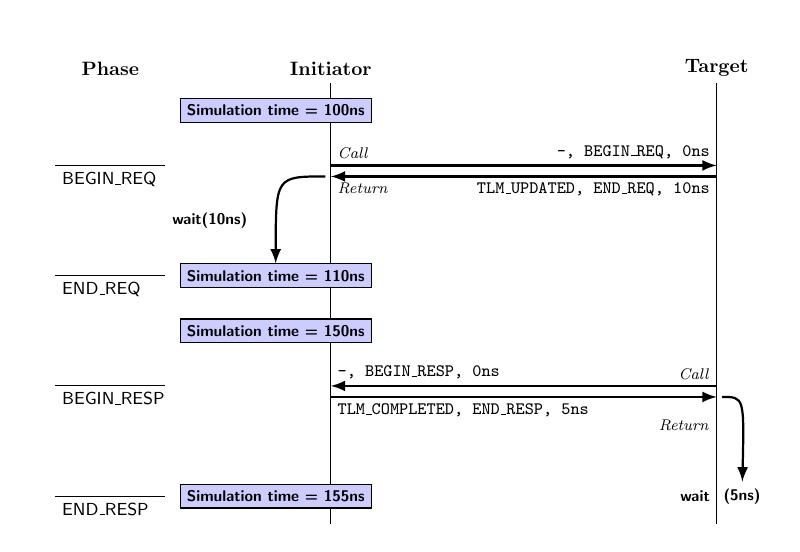
\begin{tikzpicture}[transform shape,scale=0.7]
		\clip (1.5,11) rectangle (15,20);
%		\draw[help lines] (0,0) grid (16,20);
		\path (3,19) coordinate (phase);
		\path (7,0) coordinate (llb);
		\path (7,19) coordinate (llt);
		\path (14,0) coordinate (rlb);
		\path (14,19) coordinate (rlt);
		
		\path (6,18.5) coordinate (100ns);
		\path (2,17.5) coordinate (breq_l);
		\path (4,17.5) coordinate (breq_r);
		\path (7,17.5) coordinate (breq_call_l);
		\path (14,17.5) coordinate (breq_call_r);
		\path (7,17.3) coordinate (breq_ret_l);
		\path (14,17.3) coordinate (breq_ret_r);
		
		\path (4,16.5) coordinate (wait10ns);

		\path (6,15.5) coordinate (110ns);
		\path (2,15.5) coordinate (ereq_l);
		\path (4,15.5) coordinate (ereq_r);

		\path (6,14.5) coordinate (150ns);
		\path (2,13.5) coordinate (bresp_l);
		\path (4,13.5) coordinate (bresp_r);
		\path (7,13.5) coordinate (bresp_call_l);
		\path (14,13.5) coordinate (bresp_call_r);
		\path (7,13.3) coordinate (bresp_ret_l);
		\path (14,13.3) coordinate (bresp_ret_r);

		\path (6,11.5) coordinate (155ns);
		\path (2,11.5) coordinate (eresp_l);
		\path (4,11.5) coordinate (eresp_r);
		\path (14,11.5) coordinate (wait5ns);

		\draw (phase) node[above] {\textbf{Phase}};
		\draw (llb) -- (llt)
			node[above] {\textbf{Initiator}};
		\draw (rlb) -- (rlt)
			node[above] {\textbf{Target}};

		\draw (100ns) node [rectangle,draw,fill=blue!20] {\footnotesize \textsf{\textbf{Simulation time = 100ns}}};
		\draw (breq_l) node[below right] {\small \textsf{BEGIN\_REQ}} -- (breq_r);
		\draw[thick,-latex] (breq_call_l) -- (breq_call_r);
		\draw (breq_call_l) node[above right] {\footnotesize \emph{Call}};
		\draw (breq_call_r) node[above left] {\small \texttt{\textbf{-, BEGIN\_REQ, 0ns}}};
		\draw[thick,latex-] (breq_ret_l) -- (breq_ret_r);
		\draw (breq_ret_l) node[below right] {\footnotesize \emph{Return}};
		\draw (breq_ret_r) node[below left] {\small \texttt{\textbf{TLM\_UPDATED, END\_REQ, 10ns}}};

		\draw (wait10ns) node(wait10ns_rect) [right] {\footnotesize \textsf{\textbf{wait(10ns)}}};
		
		\draw (110ns) node(sim110ns) [rectangle,draw,fill=blue!20] {\footnotesize \textsf{\textbf{Simulation time = 110ns}}};
		\path (breq_ret_l) +(-1,0) coordinate (control);
		\draw[thick,-latex] (breq_ret_l) +(-0.1,0) .. controls (control) .. (sim110ns)[above];

		\draw (ereq_l) node[below right] {\small \textsf{END\_REQ}} -- (ereq_r);

		\draw (150ns) node [rectangle,draw,fill=blue!20] {\footnotesize \textsf{\textbf{Simulation time = 150ns}}};
		\draw (bresp_l) node[below right] {\small \textsf{BEGIN\_RESP}} -- (bresp_r);
		\draw[thick,latex-] (bresp_call_l) -- (bresp_call_r);
		\draw (bresp_call_r) node[above left] {\footnotesize \emph{Call}};
		\draw (bresp_call_l) node[above right] {\small \texttt{\textbf{-, BEGIN\_RESP, 0ns}}};
		\draw[thick,-latex] (bresp_ret_l) -- (bresp_ret_r);
		\draw (bresp_ret_r) +(0,-0.3) node[below left] {\footnotesize \emph{Return}};
		\draw (bresp_ret_l) node[below right] {\small \texttt{\textbf{TLM\_COMPLETED, END\_RESP, 5ns}}};

		\draw (155ns) node [rectangle,draw,fill=blue!20] {\footnotesize \textsf{\textbf{Simulation time = 155ns}}};
		\draw (eresp_l) node[below right] {\small \textsf{END\_RESP}} -- (eresp_r);

		\draw (wait5ns) node [left] {\footnotesize \textsf{\textbf{wait}}};
		\draw (wait5ns) node(wait5ns_rect) [right] {\footnotesize \textsf{\textbf{(5ns)}}};
		\path (bresp_ret_r) +(0.5,0) coordinate (control);
		\draw[thick,-latex] (bresp_ret_r) +(0.1,0) .. controls (control) .. (wait5ns_rect)[above];
	\end{tikzpicture}
	\end{center}
\end{figure}

\end{frame}

}

\mode<article>{
Figure~\ref{fig:chart_at_with_timing_annotation} shows the message exchange that occur when using the approximately-timed coding style with timing annotations.

\begin{figure}[h]
	\begin{center}
	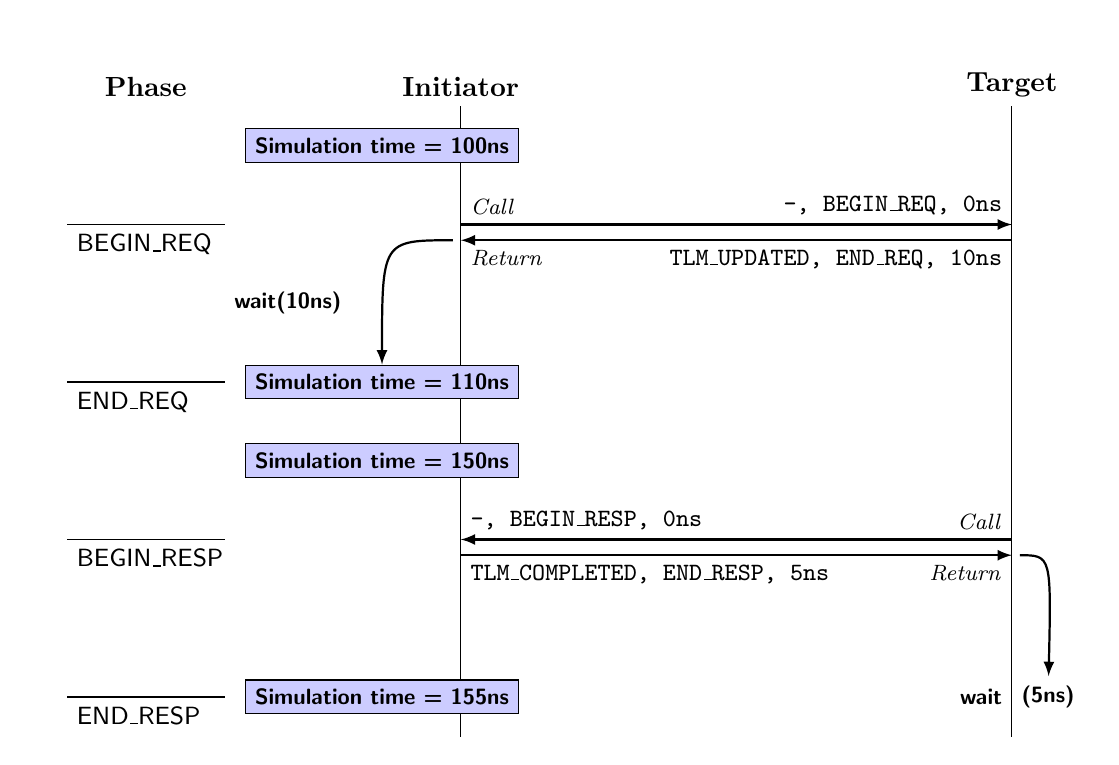
\begin{tikzpicture}
		\clip (1.5,11) rectangle (15,20);
%		\draw[help lines] (0,0) grid (16,20);
		\path (3,19) coordinate (phase);
		\path (7,0) coordinate (llb);
		\path (7,19) coordinate (llt);
		\path (14,0) coordinate (rlb);
		\path (14,19) coordinate (rlt);
		
		\path (6,18.5) coordinate (100ns);
		\path (2,17.5) coordinate (breq_l);
		\path (4,17.5) coordinate (breq_r);
		\path (7,17.5) coordinate (breq_call_l);
		\path (14,17.5) coordinate (breq_call_r);
		\path (7,17.3) coordinate (breq_ret_l);
		\path (14,17.3) coordinate (breq_ret_r);
		
		\path (4,16.5) coordinate (wait10ns);

		\path (6,15.5) coordinate (110ns);
		\path (2,15.5) coordinate (ereq_l);
		\path (4,15.5) coordinate (ereq_r);

		\path (6,14.5) coordinate (150ns);
		\path (2,13.5) coordinate (bresp_l);
		\path (4,13.5) coordinate (bresp_r);
		\path (7,13.5) coordinate (bresp_call_l);
		\path (14,13.5) coordinate (bresp_call_r);
		\path (7,13.3) coordinate (bresp_ret_l);
		\path (14,13.3) coordinate (bresp_ret_r);

		\path (6,11.5) coordinate (155ns);
		\path (2,11.5) coordinate (eresp_l);
		\path (4,11.5) coordinate (eresp_r);
		\path (14,11.5) coordinate (wait5ns);

		\draw (phase) node[above] {\textbf{Phase}};
		\draw (llb) -- (llt)
			node[above] {\textbf{Initiator}};
		\draw (rlb) -- (rlt)
			node[above] {\textbf{Target}};

		\draw (100ns) node [rectangle,draw,fill=blue!20] {\footnotesize \textsf{\textbf{Simulation time = 100ns}}};
		\draw (breq_l) node[below right] {\small \textsf{BEGIN\_REQ}} -- (breq_r);
		\draw[thick,-latex] (breq_call_l) -- (breq_call_r);
		\draw (breq_call_l) node[above right] {\footnotesize \emph{Call}};
		\draw (breq_call_r) node[above left] {\small \texttt{\textbf{-, BEGIN\_REQ, 0ns}}};
		\draw[thick,latex-] (breq_ret_l) -- (breq_ret_r);
		\draw (breq_ret_l) node[below right] {\footnotesize \emph{Return}};
		\draw (breq_ret_r) node[below left] {\small \texttt{\textbf{TLM\_UPDATED, END\_REQ, 10ns}}};

		\draw (wait10ns) node(wait10ns_rect) [right] {\footnotesize \textsf{\textbf{wait(10ns)}}};
		
		\draw (110ns) node(sim110ns) [rectangle,draw,fill=blue!20] {\footnotesize \textsf{\textbf{Simulation time = 110ns}}};
		\path (breq_ret_l) +(-1,0) coordinate (control);
		\draw[thick,-latex] (breq_ret_l) +(-0.1,0) .. controls (control) .. (sim110ns)[above];

		\draw (ereq_l) node[below right] {\small \textsf{END\_REQ}} -- (ereq_r);

		\draw (150ns) node [rectangle,draw,fill=blue!20] {\footnotesize \textsf{\textbf{Simulation time = 150ns}}};
		\draw (bresp_l) node[below right] {\small \textsf{BEGIN\_RESP}} -- (bresp_r);
		\draw[thick,latex-] (bresp_call_l) -- (bresp_call_r);
		\draw (bresp_call_r) node[above left] {\footnotesize \emph{Call}};
		\draw (bresp_call_l) node[above right] {\small \texttt{\textbf{-, BEGIN\_RESP, 0ns}}};
		\draw[thick,-latex] (bresp_ret_l) -- (bresp_ret_r);
		\draw (bresp_ret_r) node[below left] {\footnotesize \emph{Return}};
		\draw (bresp_ret_l) node[below right] {\small \texttt{\textbf{TLM\_COMPLETED, END\_RESP, 5ns}}};

		\draw (155ns) node [rectangle,draw,fill=blue!20] {\footnotesize \textsf{\textbf{Simulation time = 155ns}}};
		\draw (eresp_l) node[below right] {\small \textsf{END\_RESP}} -- (eresp_r);

		\draw (wait5ns) node [left] {\footnotesize \textsf{\textbf{wait}}};
		\draw (wait5ns) node(wait5ns_rect) [right] {\footnotesize \textsf{\textbf{(5ns)}}};
		\path (bresp_ret_r) +(0.5,0) coordinate (control);
		\draw[thick,-latex] (bresp_ret_r) +(0.1,0) .. controls (control) .. (wait5ns_rect)[above];
	\end{tikzpicture}
	\end{center}
	\caption{Approximately-timed coding style with timing annotation message chart.}
	\label{fig:chart_at_with_timing_annotation}
\end{figure}
}

% to do if we have time
% \subsection{Loosely- to approximately-timed adapter}

% to do if we have time
% \subsection{Approximately-timed initiator to loosely-timed target}
